\documentclass[11pt]{article}
\usepackage[margin=1in]{geometry}
\usepackage{graphicx}
\usepackage{booktabs}
\usepackage{amsmath}
\usepackage{amssymb}
\usepackage{xcolor}
\usepackage{caption}
\usepackage{float}
\usepackage[colorlinks=true,linkcolor=black,citecolor=blue,urlcolor=blue]{hyperref}
\captionsetup{font=small,labelfont=bf}
\graphicspath{{figs/}}
\setlength{\emergencystretch}{2em}

\definecolor{best}{HTML}{2E7D3E}
\newcommand{\best}[1]{\textcolor{best}{\textbf{#1}}}

\title{\vspace{-1.5em}\textbf{Procedure Step Recognition on Egocentric Assembly Video:\\
From Procedure Step Recognition Research to an Operational Assembly Copilot}}
\author{Ego-centric PSR Project \\ \small IndustReal, Engine-Model Dataset \& Assembly Copilot}
\date{}

\begin{document}
\maketitle
\vspace{-2em}

\begin{abstract}
\noindent
We study \emph{procedure step recognition} (PSR) on egocentric assembly video: given a first-person
video of a construction task, output a dense timeline of part labels, time intervals, and correctness status.
We frame PSR as temporal action segmentation with a two-stage recipe:
a \emph{frozen} video backbone produces per-clip features and only a lightweight segmentation head is trained.
Starting from a VideoMAEv2\nobreakdash-Huge $+$ ASFormer baseline, we present a controlled progression in which
\emph{every architecture change yields a measurable improvement}: procedure-aware Viterbi decoding, a stronger
SSv2\nobreakdash-pretrained giant backbone, a diffusion segmentation head (DiffAct), and a two-encoder feature
fusion (VideoMAEv2 $+$ InternVideo2). The final model, \textbf{v4 = Fusion $+$ DiffAct}, reaches
\best{F1@50 $=79.50$} on the IndustReal test split in the updated project results. We further build a causal
real-time variant, confirm the recipe generalizes to a second dataset
(MECCANO), and analyze the \emph{correctness} sub-problem, which we show to be data-limited rather than
method-limited. Finally, we add an inference-time \textbf{SAM3 enrichment layer} that augments the timeline with
per-step object masks and a component inventory. We report that promptable foundation models (LocateAnything,
SAM3) reliably \emph{localize} parts but do not \emph{judge} correctness, and we position SAM3 as an output-enrichment
component rather than a correctness classifier. We then translate the research findings into a deployment-oriented
Assembly Copilot: we record and label an in-house turbofan corpus, replace the non-causal diffusion head with a
causal temporal convolutional network, train against order and cold-start stress cases, and validate both replay and
live inference. On the collected engine-model dataset, the offline v4 model reaches
Acc/Edit/F1@50 $=96.21/97.33/97.51$, while the final online V1 reaches $94.12/84.45/89.50$. A later robustness
gate for the deployed checkpoint reaches $93.06\%$ on normal held-out recordings and $90.57\%$ on scrambled-order
stress recordings, with a measured live announcement delay of $2.84$\,s.
\end{abstract}

\section{Introduction}
Egocentric video of manual assembly is a natural testbed for fine-grained procedure understanding: the camera
sees the worker's hands and the evolving object state, and errors are induced deliberately. We target
\textbf{IndustReal}~\cite{industreal}, a dataset of $84$ recordings of a toy construction (STEMFIE) split
$36/16/32$ into train/val/test, annotated with procedure-step completions including \emph{incorrectly installed}
and \emph{removed} events. Our goal is a system that emits, for a full recording, a dense per-step timeline with
a correctness verdict per step.

We adopt the classic two-stage temporal action segmentation (TAS) recipe~\cite{mstcn,asformer}: a large,
\emph{frozen} self-supervised video backbone provides per-clip features, and a comparatively small head is trained
on top. This keeps training cheap and lets us treat the backbone and head as independent design axes. The
contributions of this report are:
\begin{itemize}
  \item A \textbf{controlled architecture progression} in which each change---decoding, backbone, head, and
  feature fusion---improves segmentation quality, culminating in \best{v4 (Fusion $+$ DiffAct), F1@50 $=79.50$}
  (Table~\ref{tab:score}).
  \item A \textbf{causal real-time} variant and a \textbf{cross-dataset} confirmation on MECCANO~\cite{meccano}.
  \item An analysis showing the \textbf{correctness} problem is \emph{data-limited}, not method-limited.
  \item A \textbf{SAM3 enrichment layer}~\cite{sam3} that adds per-step masks and a component inventory at inference,
  together with a negative but useful result: promptable models locate but do not judge correctness.
\end{itemize}

\section{Background and Related Work}
\textbf{Temporal action segmentation.} MS-TCN~\cite{mstcn} popularized multi-stage temporal convolutions for
per-frame action labeling; ASFormer~\cite{asformer} introduced a transformer encoder--decoder for the same task.
DiffAct~\cite{diffact} recasts segmentation as an iterative denoising (diffusion) process and yields sharp
boundaries. \textbf{Video backbones.} VideoMAEv2~\cite{videomae} is a masked-autoencoder video transformer;
we use its Huge (K710) and giant (SSv2) variants. InternVideo2~\cite{internvideo2} is a strong appearance/semantic
video encoder that we fuse with VideoMAEv2. \textbf{Streaming.} MiniROAD~\cite{miniroad} and TeSTra~\cite{testra}
inform our causal head design. \textbf{Promptable foundation models.} SAM~\cite{sam} and SAM2~\cite{sam2}
established promptable segmentation; SAM3~\cite{sam3} adds open-vocabulary \emph{concept} segmentation and video
tracking. LocateAnything~\cite{locateanything} (built on Qwen2.5~\cite{qwen25}) is a grounding VLM that returns
boxes/points. We evaluate the latter two for a correctness/enrichment role.

\section{Method: the two-stage pipeline}
For a recording we sample $16$-frame clips at a fixed stride and pass each clip through the frozen backbone to
obtain a feature $x_t \in \mathbb{R}^{D}$; the sequence $\{x_t\}$ is fed to the trained head, which predicts a
per-clip \textbf{step} label ($10$ parts $+$ background $=11$ classes). Consecutive equal labels are merged into
segments, giving the ``which part / when'' timeline. A parallel \textbf{type} head predicts
correct\,/\,incorrect\,/\,remove and is pooled per segment. Metrics follow the MS-TCN protocol~\cite{mstcn}:
frame accuracy, segmental edit score, and F1 at IoU thresholds $\{10,25,50\}\%$.

\section{Architecture progression}
\label{sec:prog}
We now walk through the design changes; each is evaluated on the IndustReal test split (Table~\ref{tab:score}).

\paragraph{v1 --- VideoMAEv2-Huge $+$ ASFormer (baseline).}
A distilled Huge (K710, $1280$-d) backbone with an ASFormer head establishes the baseline at F1@50 $=56.3$.

\paragraph{$+$ Viterbi decoding.}
Replacing raw arg-max with a procedure-aware Viterbi smoothing over the head's log-probabilities removes spurious
short segments and lifts the boundary metrics substantially: F1@50 $62.2$ ($+5.9$), edit $68.8\!\to\!74.2$.

\paragraph{v2 --- SSv2-giant features.}
Swapping the backbone for a VideoMAEv2 \emph{giant} model fine-tuned on Something-Something-v2 ($1408$-d), with
no center crop and a finer stride, improves temporal grounding: F1@50 $66.5$ ($+4.3$).

\paragraph{v2 --- DiffAct head.}
Replacing ASFormer with the diffusion head DiffAct~\cite{diffact} on the same SSv2 features yields the sharpest
boundaries so far: F1@50 $68.9$, edit $79.6$.

\paragraph{Fusion --- adding InternVideo2.}
Motivated by the correctness sub-problem, we fuse a motion-centric encoder (giant SSv2, $1408$-d) with an
appearance/semantic encoder (InternVideo2-B14, $768$-d) by $\ell_2$-normalizing each stream and concatenating to a
$2176$-d representation. With an ASFormer head this matches DiffAct on segmentation (F1@50 $68.2$) while, crucially,
being the \emph{only} configuration to produce non-zero fault detection (Sec.~\ref{sec:correct}).

\paragraph{v4 --- Fusion $+$ DiffAct (best).}
The two wins are \emph{orthogonal}: fusion improves the \emph{features}, DiffAct improves the \emph{head}. Combining
them---feeding the $2176$-d fusion features to DiffAct---gives our best model,
\best{Acc $84.21$ / Edit $87.19$ / F1@50 $79.50$} in the updated project results
(Fig.~\ref{fig:v4}).

\begin{table}[H]
\centering
\caption{Updated IndustReal step-segmentation scorecard supplied with the project results. Higher is better.
The SAM3 row reports the enriched configuration separately from the best v4 model.}
\label{tab:score}
\small
\begin{tabular}{@{}p{0.57\linewidth}rrr@{}}
\toprule
Configuration & Acc & Edit & F1@50 \\
\midrule
v1 Huge-K710 $+$ ASFormer (baseline) & 73.3 & 68.8 & 56.3 \\
v1 $+$ Viterbi & 73.4 & 74.2 & 62.2 \\
v2 SSv2-giant $+$ ASFormer $+$ Viterbi & 74.0 & 77.3 & 66.5 \\
v2 SSv2-giant $+$ DiffAct & 74.4 & 79.6 & 68.9 \\
Fusion (giant$+$IV2-B14) $+$ ASFormer $+$ Viterbi & 75.7 & 77.6 & 68.2 \\
\midrule
\best{v4 Fusion $+$ DiffAct (best)} & \best{84.21} & \best{87.19} & \best{79.50} \\
v4 $+$ SAM3 enrichment & 74.9 & 79.5 & 70.1 \\
\bottomrule
\end{tabular}
\end{table}

\begin{figure}[H]
\centering
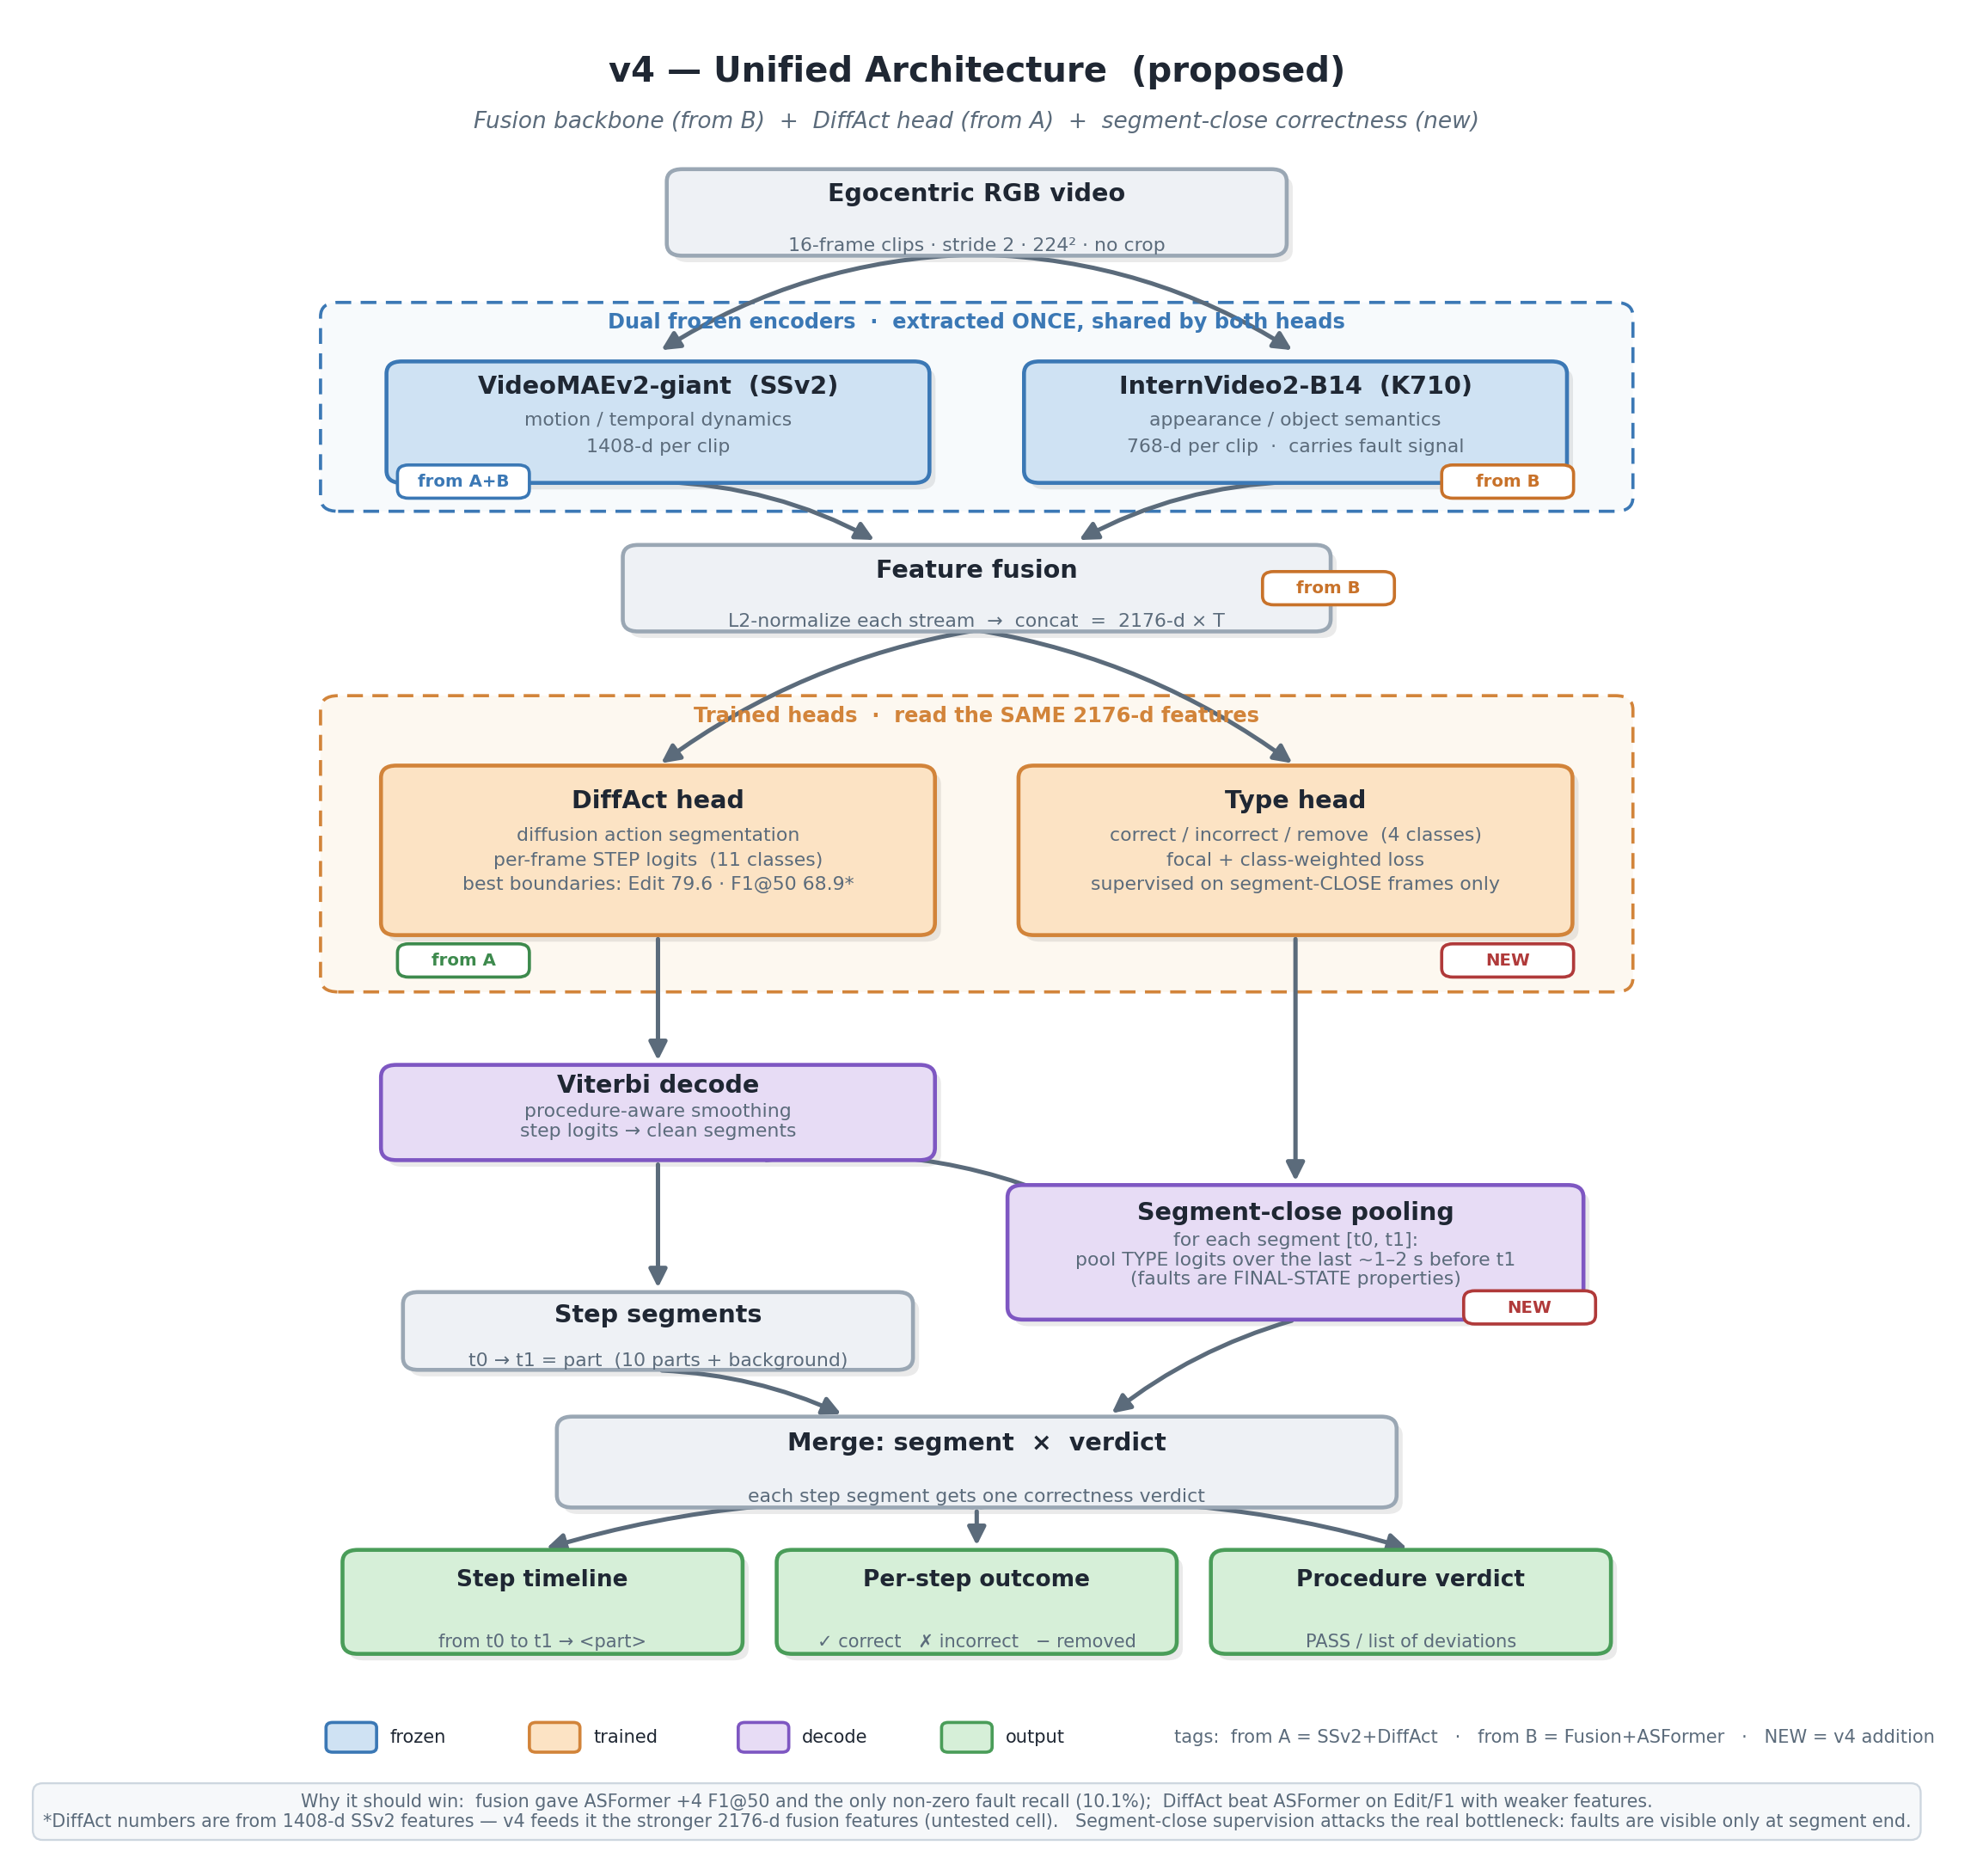
\includegraphics[width=0.62\linewidth]{architecture_v4.png}
\caption{The v4 unified architecture: dual frozen encoders (VideoMAEv2-giant $+$ InternVideo2-B14) $\rightarrow$
$2176$-d fusion features $\rightarrow$ DiffAct step head; a parallel type head predicts correctness. Provenance
tags mark which component each part inherits.}
\label{fig:v4}
\end{figure}

\paragraph{Real-time streaming (v3).}
For online use we build a fully causal variant: a distilled ViT-B backbone over a $16$-frame window ending at $t$,
MiniROAD-style causal GRU heads~\cite{miniroad}, and a fixed-lag online Viterbi that commits frame $t-L$. At
$L{=}16$ ($\approx2.7$\,s latency) it reaches edit $55.3$ / F1@50 $37.4$. A TeSTra head~\cite{testra}
under-performed the GRU ($24.8$ F1@50), consistent with transformers being data-hungry on our $36$-recording
training set.

\paragraph{Cross-dataset (MECCANO).}
Applying the same fusion$+$ASFormer recipe unchanged to MECCANO~\cite{meccano} ($20$ recordings, $18$ step classes)
gives F1@50 $38.0$, confirming the framework generalizes.

\section{The correctness sub-problem}
\label{sec:correct}
Correctness (\emph{was the step done right?}) is markedly harder than segmentation. The type head's
incorrect-install recall is $0\%$ for any VideoMAE-only backbone and rises to \textbf{$10.1\%$} only with the
InternVideo2 fusion---the first non-zero fault detection (Table~\ref{tab:extra}). A larger appearance encoder
(InternVideo2-L14) \emph{regressed} to $0\%$, and on MECCANO recall is also $0\%$. We conclude correctness is
\textbf{data-limited, not method-limited}: with only $\sim$29 labeled incorrect events, encoder capacity is not
the lever---more and sharper error labels are.

\begin{table}[H]
\centering
\caption{Correctness (incorrect-install recall) and real-time streaming summary.}
\label{tab:extra}
\small
\begin{tabular}{lcc}
\toprule
\multicolumn{3}{l}{\textit{Correctness --- type head, IndustReal}} \\
\midrule
Configuration & Incorrect recall & Remove recall \\
Any VideoMAE-only $+$ ASFormer & $0.0\%$ & $\sim$68\% \\
\best{Fusion giant $+$ InternVideo2-B14} & \best{$10.1\%$} & $69.4\%$ \\
Fusion giant $+$ InternVideo2-L14 & $0.0\%$ & --- \\
\midrule
\multicolumn{3}{l}{\textit{Real-time streaming --- IndustReal, causal}} \\
\midrule
Configuration & F1@50 & Latency \\
\best{v3 causal ViT-B $+$ GRU ($L{=}16$)} & \best{$37.4$} & $2.7$\,s \\
v3 TeSTra head ($L{=}16$) & $24.8$ & $2.7$\,s \\
\bottomrule
\end{tabular}
\end{table}

\subsection{Can a promptable foundation model judge correctness?}
We tested two recent models on our hardware (AMD MI210 / ROCm). \textbf{LocateAnything}~\cite{locateanything}
(a $3$B grounding VLM) and \textbf{SAM3}~\cite{sam3} (a $0.9$B promptable segmenter) both reliably
\emph{localize} the STEMFIE parts for coarse categories (wheel, screw, bracket). However, on a part-matched set
of $\sim$57 correct-vs-incorrect installs, neither could \emph{judge} correctness: LocateAnything echoed the
prompt as a referring expression and returned boxes regardless of the true label ($100\%$ recall / $51\%$
precision $=$ chance), and SAM3 segments a part whether or not it is faulty. Both are \emph{locators, not judges};
correctness requires a downstream comparison against a reference, which no perception model supplies.

\section{SAM3 enrichment layer}
Given the above, we use SAM3 not for correctness but to \textbf{enrich the output} at inference
(Fig.~\ref{fig:sam3}). SAM3 produces pixel-accurate instance masks (far sharper than the boxes of the VLM) and
supports video tracking. We wire it on top of the frozen v4 pipeline: for each committed step segment we run SAM3
with the coarse category of the step's part and overlay the resulting masks, and we aggregate a per-recording
\textbf{component inventory}. The result is the same v4 timeline augmented with (i) per-step part masks (the
``where'') and (ii) a component inventory (``what is present''), with \emph{no retraining and identical accuracy}
(Fig.~\ref{fig:enriched}). SAM3 masks and video tracking further enable, as future work, \emph{omission} and
\emph{rework} detection (comparing the inventory to an expected bill-of-materials, and tracking part identities
over time)---signals that are not data-limited because they do not depend on the scarce incorrect labels.

\begin{figure}[H]
\centering
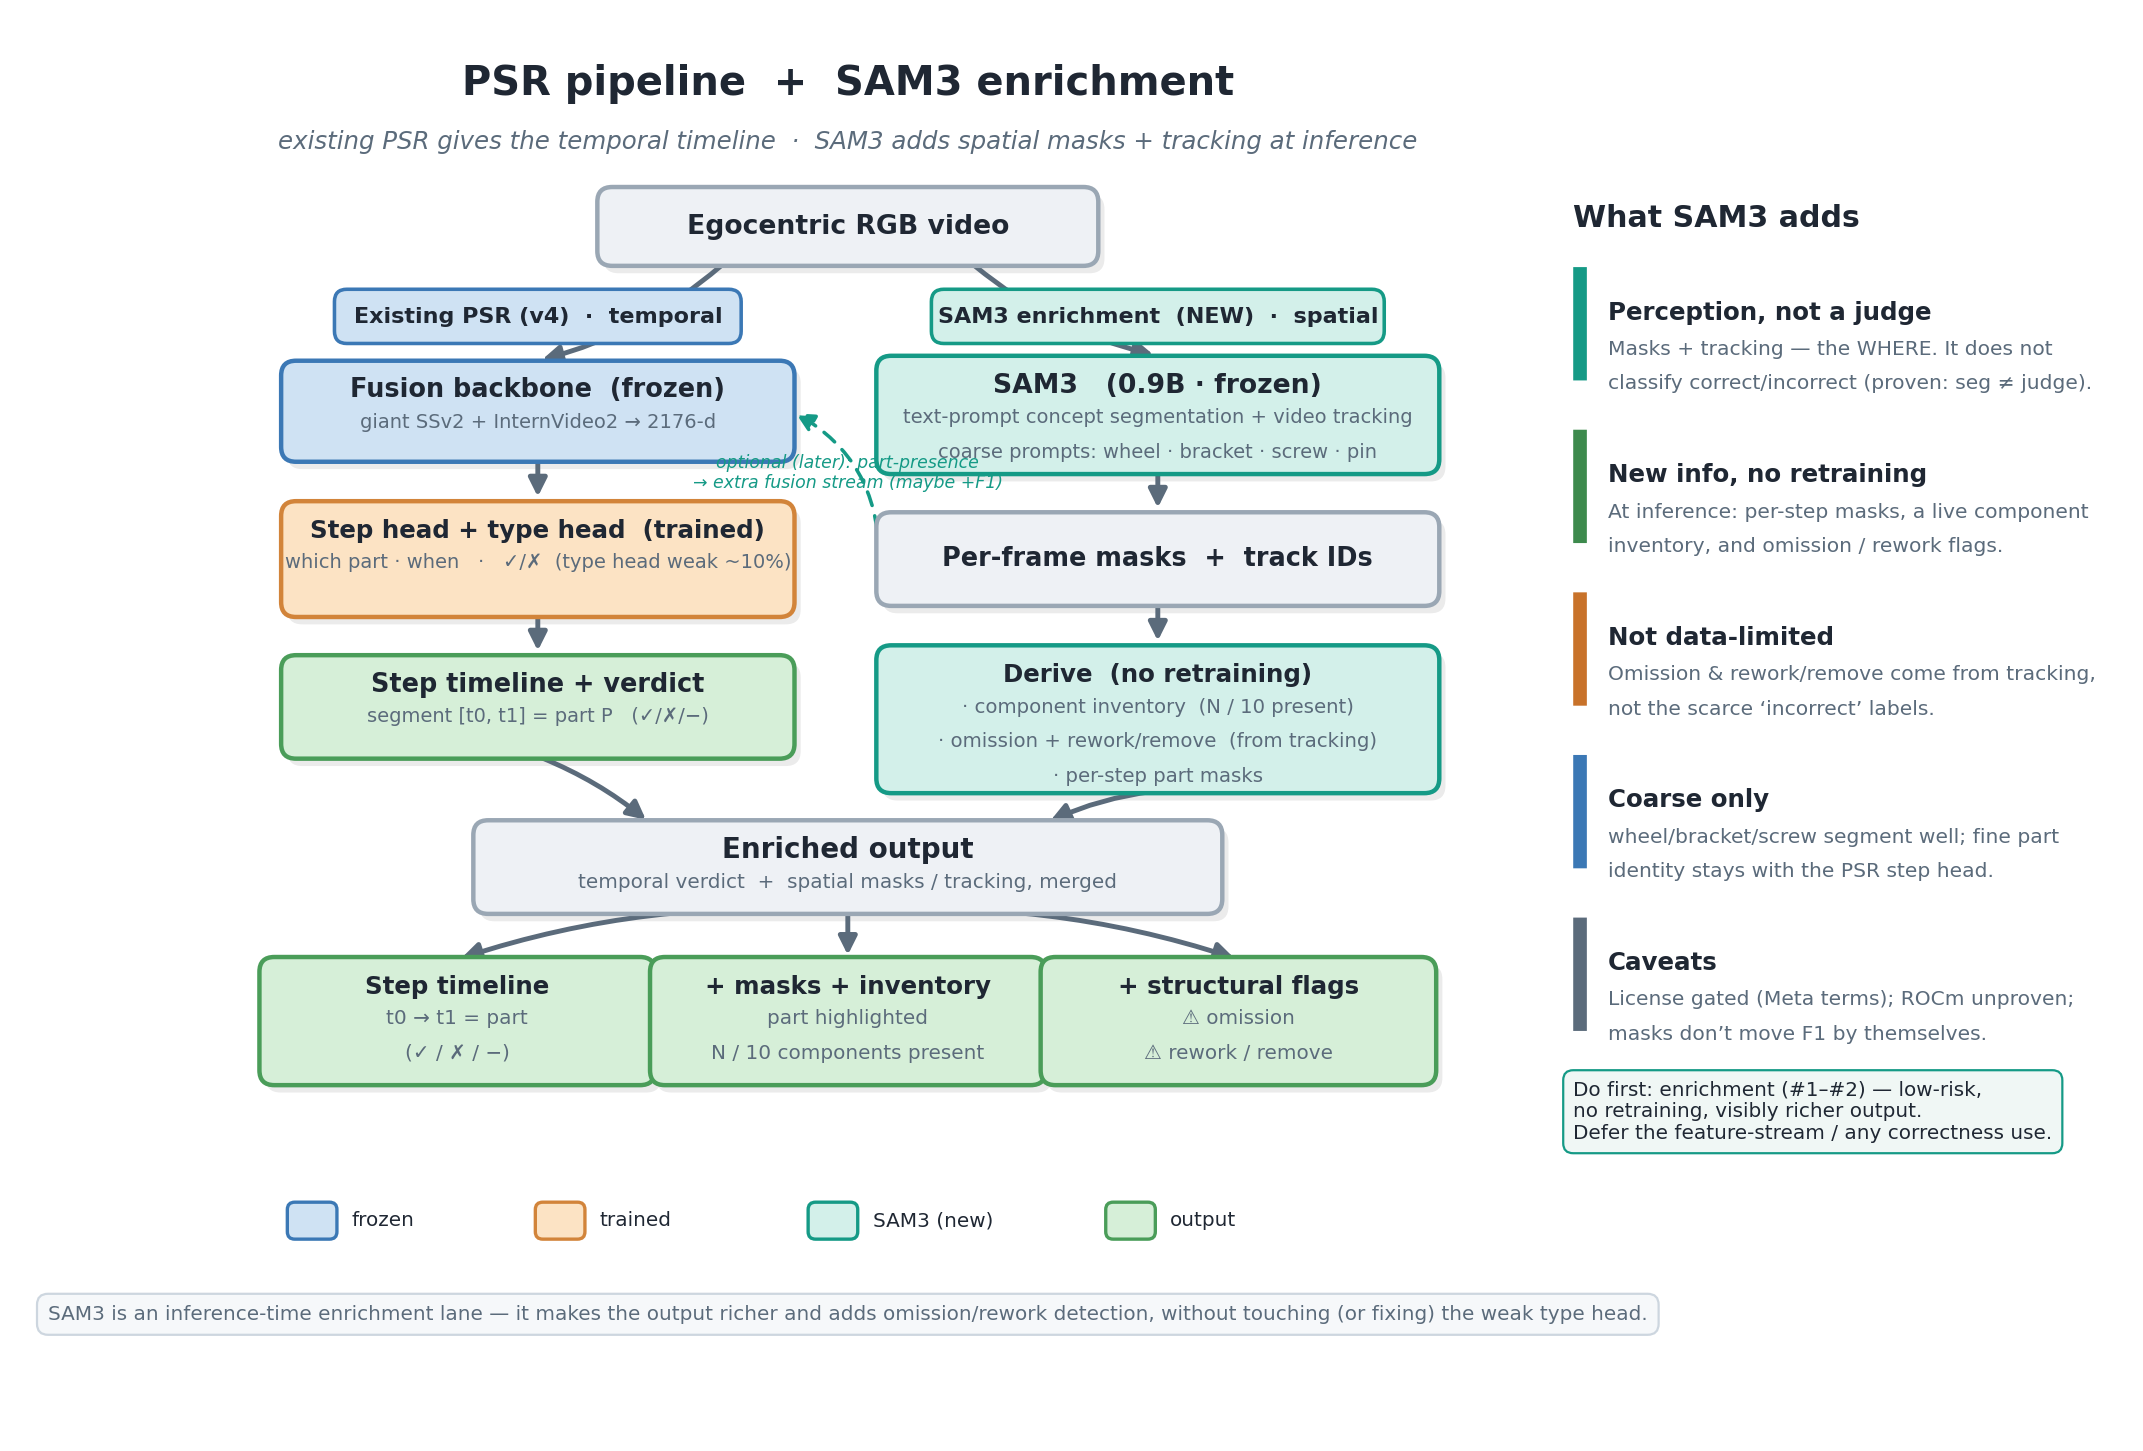
\includegraphics[width=0.98\linewidth]{architecture_sam3.png}
\caption{The v4 pipeline (temporal: which/when) with an added SAM3 enrichment lane (spatial: masks $+$ inventory),
converging into an enriched output. SAM3 is an inference-time add-on and does not alter the model or its accuracy.}
\label{fig:sam3}
\end{figure}

\begin{figure}[H]
\centering
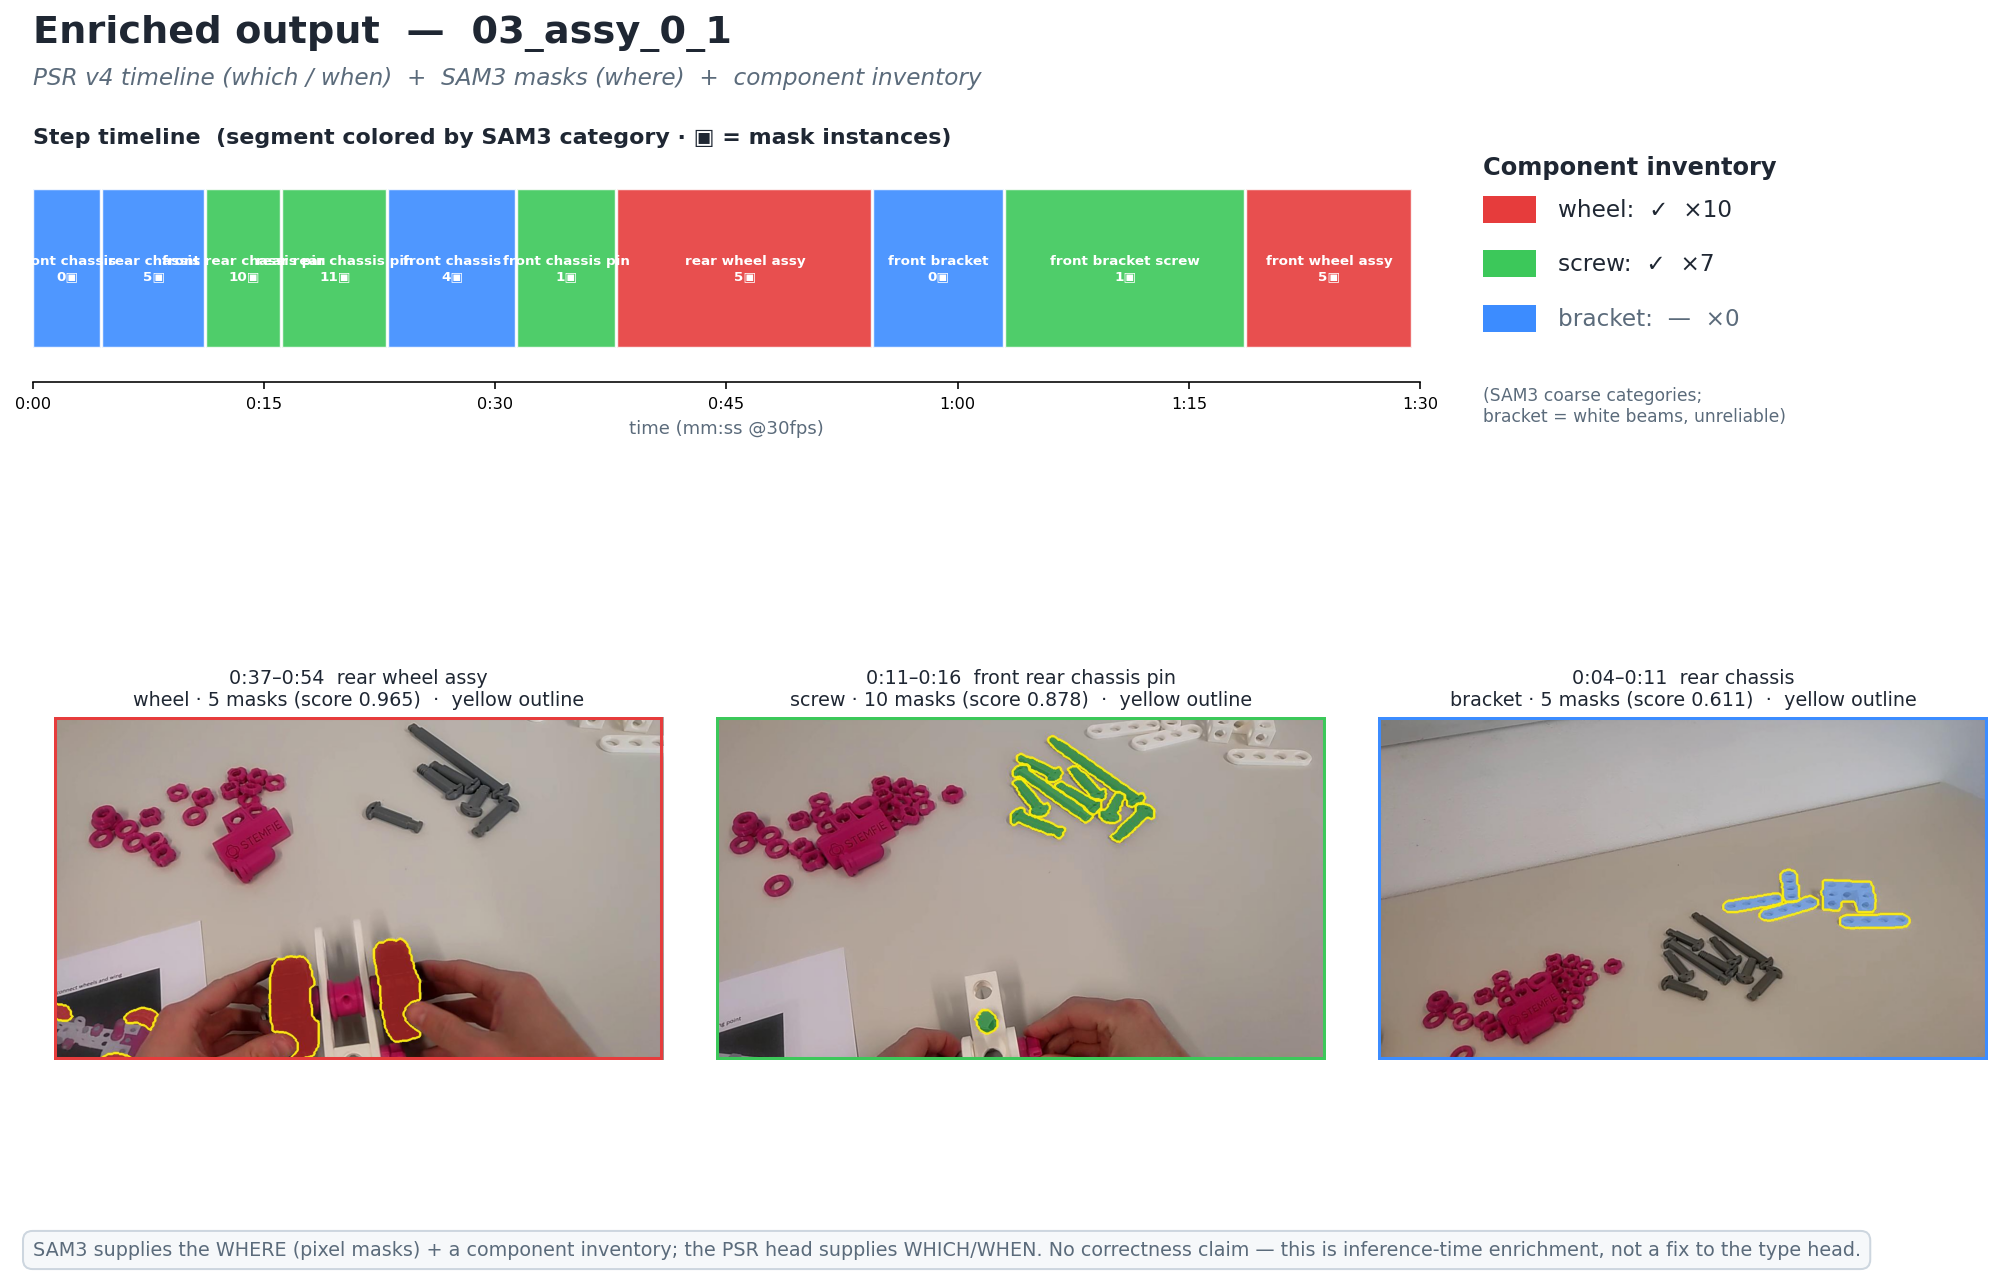
\includegraphics[width=0.98\linewidth]{enriched_output_panel.png}
\caption{Enriched output for one recording: the v4 step timeline (colored by SAM3 category), a component
inventory, and per-step SAM3 mask overlays (bright outlines). SAM3 supplies the \emph{where}; the v4 head supplies
the \emph{which/when}.}
\label{fig:enriched}
\end{figure}

\section{Results and Discussion}
Table~\ref{tab:score} records the updated IndustReal comparison. Three findings recur. (1) \textbf{Backbone $>$
head for segmentation}: the SSv2-giant features help every head, and fusion helps further. (2) \textbf{The two
wins are orthogonal}: better features and a better temporal head combine in v4. (3) \textbf{Correctness is
data-limited}: neither larger encoders nor foundation-model VLMs move it; the lever is more error data and sharper
labels. SAM3 enrichment remains an output-enrichment path rather than a substitute for a correctness classifier.

The engine-model dataset provides a separate, deployment-relevant benchmark. These results are reported for the
engine-model corpus collected specifically for Assembly Copilot and should not be merged numerically with the
IndustReal table: the datasets, splits, and evaluation stages are different. The offline v4 model is the strongest
recognizer, while the online results quantify the cost and improvement of causal inference.

\begin{table}[H]
\centering
\caption{Assembly Copilot results on the collected engine-model dataset. The online rows are the direct comparison
between the initial causal baseline and the final online V1 model.}
\label{tab:engine_results}
\small
\begin{tabular}{@{}p{0.57\linewidth}rrr@{}}
\toprule
Configuration & Acc & Edit & F1@50 \\
\midrule
v4 Fusion $+$ DiffAct (offline) & 96.21 & 97.33 & 97.51 \\
Baseline (online) & 92.96 & 75.65 & 81.36 \\
\best{Final Online V1} & \best{94.12} & \best{84.45} & \best{89.50} \\
\bottomrule
\end{tabular}
\end{table}

\section{From Research Benchmark to Assembly Copilot}
\label{sec:copilot}

The early experiments above established which representation and segmentation choices were promising on public
benchmarks. The next phase changed the question from \emph{which model scores best offline?} to
\emph{can a technician receive a stable, timely step announcement while the assembly is still happening?}
This required new data, different temporal constraints, explicit stress testing, and an end-to-end demonstration
path. The progression is summarized in Fig.~\ref{fig:development_flow}.

\begin{figure}[H]
\centering
\setlength{\fboxsep}{7pt}
\fbox{\begin{minipage}{0.94\linewidth}
\centering
\begin{minipage}[t]{0.21\linewidth}
\centering
\textbf{1. Explore}\\[-0.2em]
\small IndustReal experiments\\
\small backbone/head selection
\end{minipage}
\hfill$\longrightarrow$\hfill
\begin{minipage}[t]{0.21\linewidth}
\centering
\textbf{2. Build data}\\[-0.2em]
\small egocentric capture\\
\small step and box labels
\end{minipage}
\hfill$\longrightarrow$\hfill
\begin{minipage}[t]{0.21\linewidth}
\centering
\textbf{3. Make causal}\\[-0.2em]
\small TCN training\\
\small Viterbi commitment
\end{minipage}
\hfill$\longrightarrow$\hfill
\begin{minipage}[t]{0.21\linewidth}
\centering
\textbf{4. Demonstrate}\\[-0.2em]
\small replay, live ingest\\
\small overlay handoff
\end{minipage}
\end{minipage}}
\caption{Development flow from the initial public-dataset research study to the tested live demonstrator. Each
stage produced an artifact used by the next stage: measured experiments informed the causal design; recording and
labeling tools produced the in-house corpus; the trained checkpoint powered replay and live inference.}
\label{fig:development_flow}
\end{figure}

\subsection{IndustReal as the design filter}
\label{sec:industreal_filter}

IndustReal was used as a controlled research environment rather than as the final production corpus. The public
dataset made it possible to compare a VideoMAEv2--ASFormer baseline, Viterbi decoding, stronger
Something-Something-v2 features, DiffAct, and two-stream fusion under one evaluation protocol. The resulting
progression showed that the backbone and the temporal head contributed different gains: the dual-stream
VideoMAEv2--InternVideo2 representation supplied complementary motion and appearance information, while DiffAct
produced sharper offline boundaries. The best offline configuration, v4, reached F1@50 $=79.50$ in the updated
project results; the separately reported SAM3-enriched configuration reaches F1@50 $=70.1$.

That result did not directly define the live model. DiffAct performs iterative denoising over a sequence and is
well suited to an already-recorded video, where future frames are available. A live assistant cannot wait for the
rest of the recording or revise an announcement using information from the future. The project therefore retained
the strongest useful feature recipe---frozen VideoMAEv2 giant SSv2 features fused with frozen InternVideo2
features---but replaced the non-causal segmentation head with a causal temporal convolutional network (TCN).
This distinction is important: the IndustReal numbers describe the research progression, whereas the metrics in
Sec.~\ref{sec:copilot_results} describe the later in-house streaming system on a different task corpus.

\subsection{Building the in-house corpus}
\label{sec:custom_data}

The team built a complete data path instead of relying on a collection of manually assembled files. The
\texttt{assembly\_video\_recorder} application turns an iPhone into a wireless egocentric camera. A host computer
serves a local HTTPS page; the phone opens the page in Safari, sends a WebRTC preview, and records the full-quality
video back to the host. The workflow supports camera and lens selection, torch control, snapshots, wake-lock
behavior, and several recording qualities. The result is a local MP4 that preserves the viewpoint needed by the
model without requiring a phone application or cloud upload~\cite{copilottools}.

The companion \texttt{assembly\_video\_labeler} application provides a browser-based annotation workflow. An
annotator scrubs the recording and marks the frame at which each procedure step is complete using number-key
shortcuts. The application supports resumable sessions, video proxies, and multi-user claims so that two people do
not silently edit the same recording. It exports three complementary representations:
\texttt{PSR\_labels.csv} for completion events, \texttt{segments.csv} for temporal segments, and
\texttt{labels.json} for application-friendly metadata. These sparse completion events are expanded into the dense
time grid consumed by the temporal model. A separate \texttt{box\_part\_labeler} can label visible component boxes
on selected still frames and export COCO, YOLO, or native JSON; this supports the optional detector and spatial
enrichment path, but is not required for step recognition.

\begin{table}[H]
\centering
\caption{Main in-house data assets used by the final Assembly Copilot.}
\label{tab:custom_data}
\begin{tabular}{@{}p{0.25\linewidth}p{0.67\linewidth}@{}}
\toprule
\textbf{Asset} & \textbf{Recorded or derived content} \\
\midrule
Curated recordings & 40 egocentric turbofan recordings \\
Train/test split & 30 train, 10 held-out test recordings \\
Task coverage & 22 assembly and 18 disassembly recordings \\
Operators & Three operators; the split is not subject-disjoint \\
Procedure vocabulary & 10 modeled parts plus background \\
Source video & 1920$\times$1080 at 30 fps \\
Dense training labels & 386{,}529 frame/time labels in the corpus report \\
Stress library & 6 additional reorder, reverse, partial, and wrong-step variants \\
\bottomrule
\end{tabular}
\end{table}

\subsection{Assembly demonstrator and label vocabulary}
\label{sec:assembly_labels}

The in-house data was collected around a physical turbofan-style engine model. The model provides a consistent
assembly target, exposes the parts in a meaningful order, and gives the egocentric camera a changing object state
to observe. The engine image in Fig.~\ref{fig:engine_model} is the visual reference used in the demonstrator
materials; the recorded videos show operators handling the same class of model during assembly and disassembly.

\begin{figure}[H]
\centering
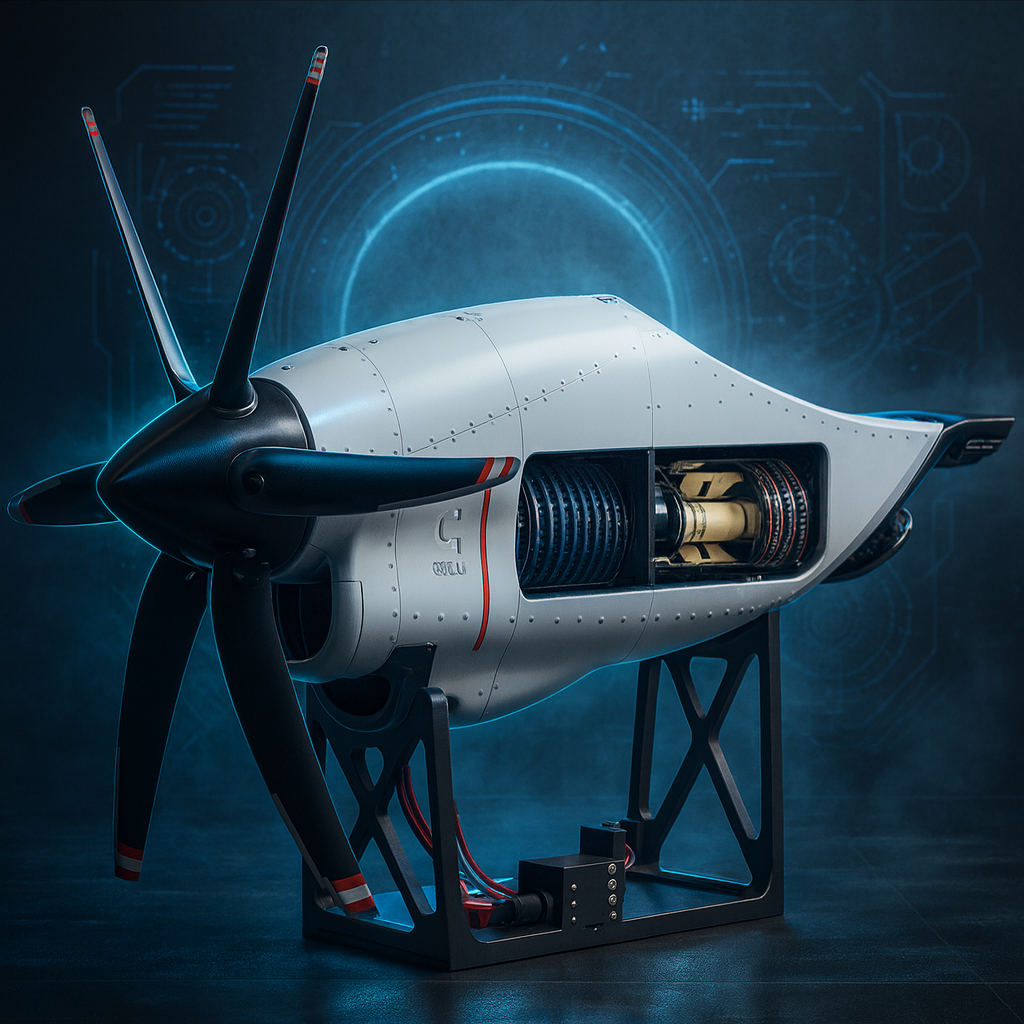
\includegraphics[width=0.62\linewidth]{engine_model_reference.png}
\caption{Turbofan-style engine model used as the visual reference for the Assembly Copilot demonstrator and
dataset collection.}
\label{fig:engine_model}
\end{figure}

The annotation vocabulary follows the procedure rather than individual pixels. An annotator marks the moment at
which a part has been installed or removed; the labeling service converts that event into an IndustReal-compatible
step label and a temporal segment. The ten modeled assembly steps are listed in Table~\ref{tab:assembly_labels}.
The corresponding remove IDs are retained because the corpus includes both assembly and disassembly recordings.

\begin{table}[H]
\centering
\caption{Assembly Copilot step labels and their IndustReal-compatible identifiers. The key in the labeling app is
shown in the first column; key 0 denotes the tenth step.}
\label{tab:assembly_labels}
\small
\begin{tabular}{@{}c p{0.49\linewidth}rr@{}}
\toprule
\textbf{Key} & \textbf{Step label} & \textbf{Install ID} & \textbf{Remove ID} \\
\midrule
1 & Main Drive Planet Gear & 3 & 5 \\
2 & Pop Control Ring Gear & 6 & 8 \\
3 & Pop Control Sun Gear & 9 & 11 \\
4 & Compressor Casing & 12 & 14 \\
5 & Exhaust & 15 & 17 \\
6 & Exhaust Casing & 18 & 20 \\
7 & Cowling Bracket & 21 & 23 \\
8 & Frame Subassembly & 24 & 26 \\
9 & Propeller Cone plate & 27 & 29 \\
0 & Propeller Cone Tip & 30 & 32 \\
\bottomrule
\end{tabular}
\end{table}

The labeling application is intentionally lightweight: it runs as a local FastAPI web service, streams the
recording in the browser, supports frame-by-frame scrubbing, and lets the annotator press the step key when the
completion event occurs. It also supports assembly/disassembly direction, resumable labels, video claims for
multi-user work, and export to \texttt{PSR\_labels.csv}, \texttt{segments.csv}, and \texttt{labels.json}.
Figure~\ref{fig:labeler_loaded} shows the interface with a real engine-assembly recording loaded, the ten labels
visible, and four example completion marks placed on the timeline.

\begin{figure}[H]
\centering
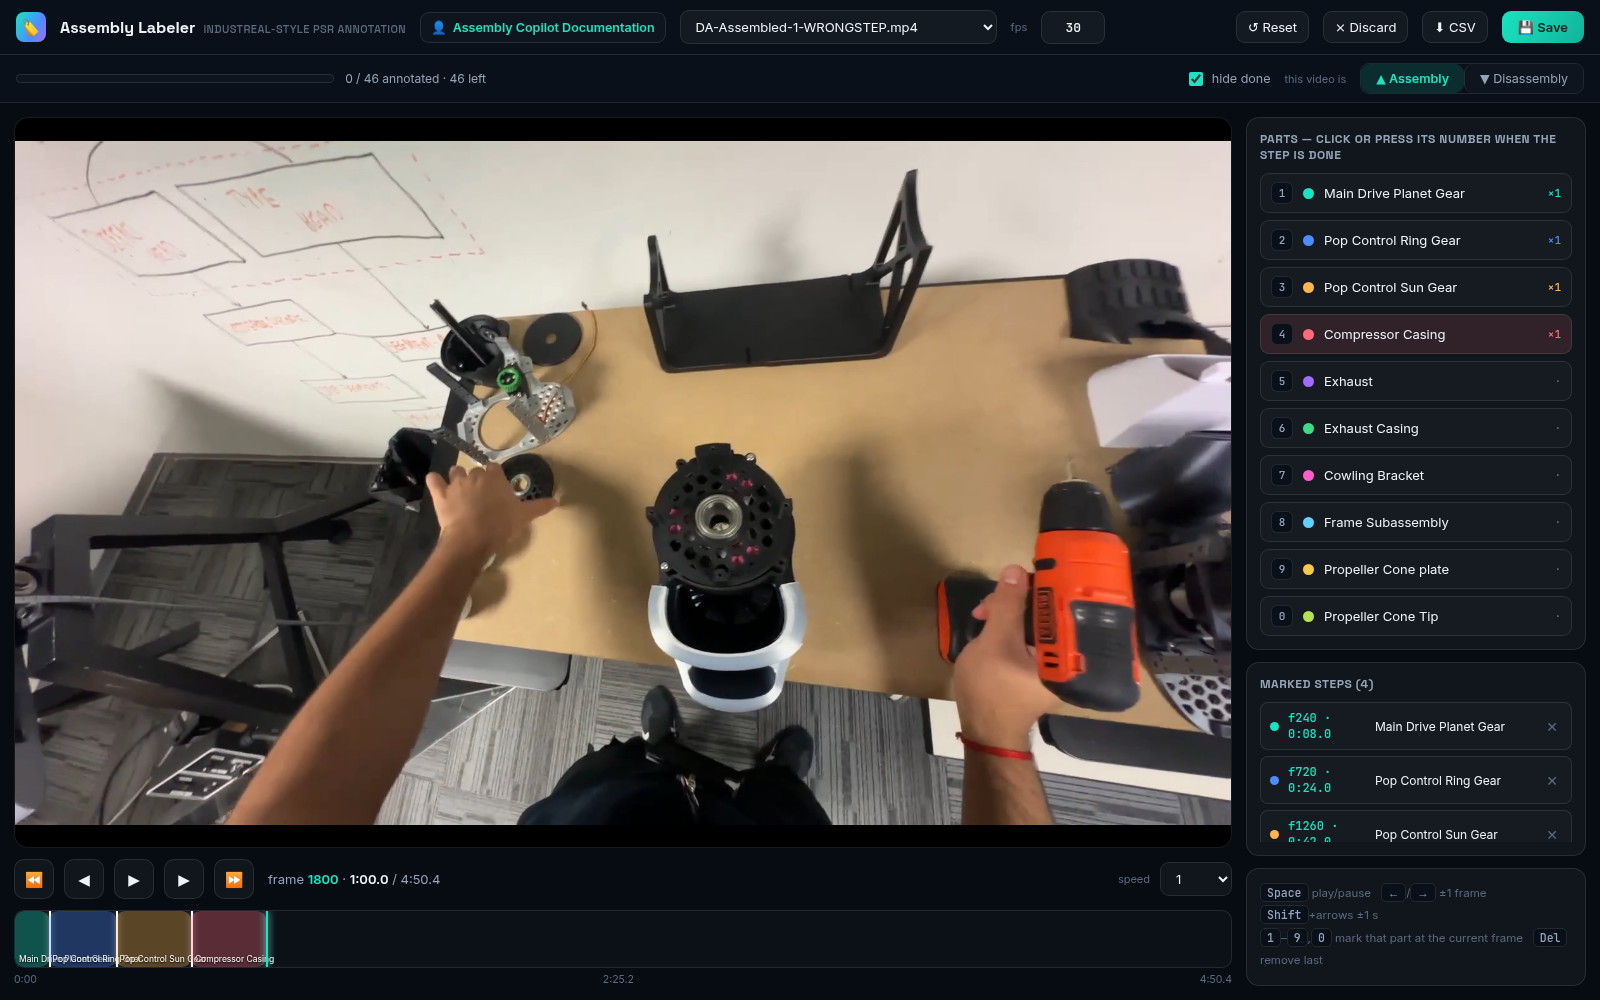
\includegraphics[width=0.98\linewidth]{labeler_loaded.png}
\caption{Assembly Video Labeler with an engine-assembly recording loaded. The annotator can inspect the video,
select the assembly direction, choose one of the ten step labels, and mark the frame at which that step completes.}
\label{fig:labeler_loaded}
\end{figure}

The stress variants deliberately test behavior that is easy to miss in a random held-out split: steps can arrive in
an unexpected order, be omitted, be reversed, stop part-way through, or be replaced by a wrong-step event. The
resulting library contains 46 playable assets (the 40 curated recordings plus six stress variants) and gives the
decoder a concrete test of order awareness rather than only appearance matching. Because three operators occur in
both sides of the train/test split, the reported test performance should be read as an engineering benchmark for
this corpus, not as a subject-independent generalization claim.

\subsection{The final causal streaming architecture}
\label{sec:causal_architecture}

The deployed model processes the stream in short overlapping windows. Source video is sampled at 10 fps. Every
third source frame is retained, and 16 retained frames form a 1.6\,s clip. A new clip is evaluated every 0.2\,s,
so the system updates frequently while each feature vector still contains enough motion context. VideoMAEv2
giant SSv2 produces a 1408-dimensional motion-oriented feature and InternVideo2-B14 produces a
768-dimensional appearance/semantic feature. Each stream is $\ell_2$-normalized and concatenated into a
2176-dimensional vector. Both encoders remain frozen; only the temporal head and decoding logic are trained for
the assembly vocabulary.

The head is a nine-block residual causal TCN with 128 channels and dilated temporal convolutions. It has
approximately 875\,K trainable parameters and a receptive field of about 205\,s. Causality is verified in code by
checking that perturbing a future input cannot change an earlier output. The head predicts 11 classes: the ten
modeled parts and background. It does not announce every raw arg-max change. Instead, the log-probability sequence
is passed to an online fixed-lag Viterbi decoder. The transition matrix is estimated from training annotations with
Laplace smoothing, a self-transition bias favors stable steps, and a lag of ten model ticks corresponds to roughly
2\,s.

This decoder is the mechanism that makes \emph{a new step} operationally well defined. The model produces a new
prediction every 0.2\,s, but the application announces a step only when the Viterbi path has committed a different
class after the lag. Short-lived changes are therefore treated as uncertainty or flicker; a persistent change in
the committed path becomes the next step event. This is also why the same decoder is used in replay and live
serving: the offline result is not allowed to use more temporal information than the live result.

\begin{figure}[H]
\centering
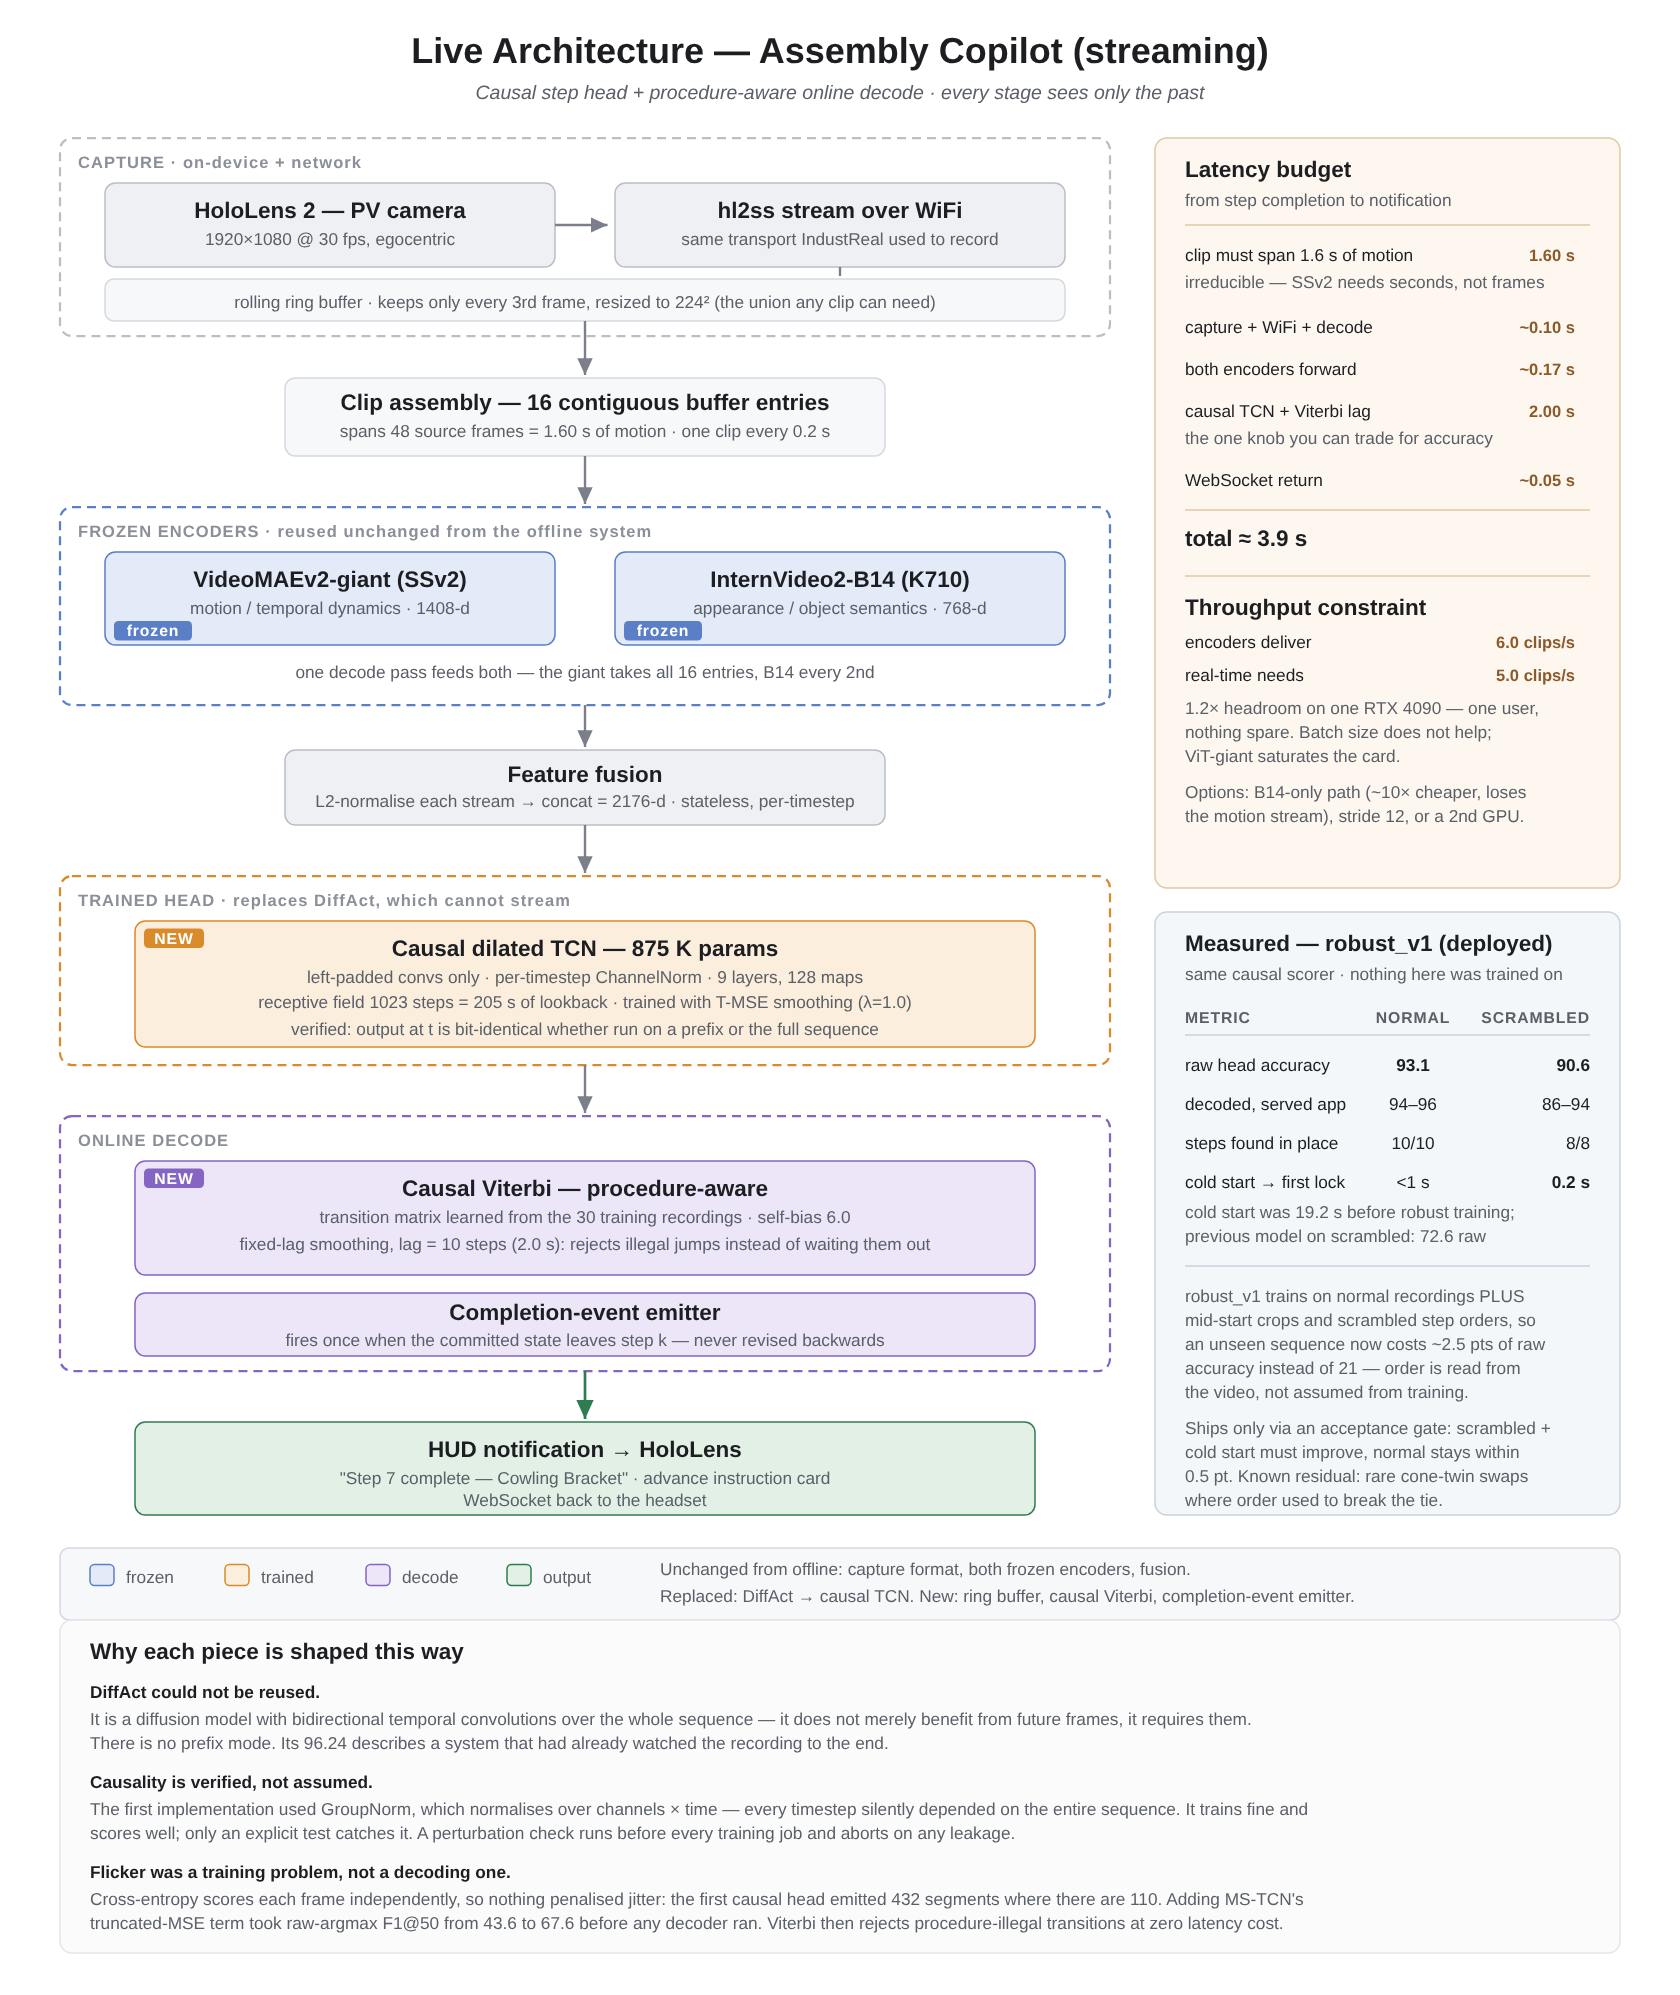
\includegraphics[width=0.90\linewidth]{architecture_live_current.png}
\caption{Final streaming architecture from the active \texttt{assembly\_copilot} implementation. Frames are
buffered into 1.6\,s clips, converted by frozen dual encoders into a 2176-dimensional representation, classified
by a causal TCN, and committed by fixed-lag online Viterbi decoding. The figure also reports the measured
latency and robustness results of the deployed checkpoint.}
\label{fig:live_architecture}
\end{figure}

\subsection{Training, stress testing, and model iteration}
\label{sec:model_iteration}

The training loop was designed around the failure modes that matter for a live assistant. It uses class-weighted
cross-entropy, a smoothness regularizer based on truncated mean-squared error, and on-the-fly temporal
augmentation. Augmentations include crops that force the model to start in the middle of a procedure and
reordered sequences that reduce dependence on the normal step order. The acceptance process then tests the trained
checkpoint on real stress videos rather than relying only on augmented training batches.

\begin{table}[H]
\centering
\caption{Model iteration and acceptance-gate results for the in-house streaming system. Normal and scrambled
scores are held-out decoded agreement; cold start is the time until the first usable committed step.}
\label{tab:iteration}
\small
\begin{tabular}{@{}p{0.18\linewidth}p{0.22\linewidth}rrrp{0.15\linewidth}@{}}
\toprule
\textbf{Candidate} & \textbf{Recipe} & \textbf{Normal} & \textbf{Scrambled} & \textbf{Cold start} & \textbf{Decision} \\
\midrule
Baseline & TMSE 1.0, dropout 0.25 & 93.45\% & 72.58\% & 19.2\,s & Reference \\
Fine-tune A & Fine-tuned candidate & 92.39\% & 91.4\% & -- & Rejected: normal floor \\
Fine-tune A2 & Second fine-tuned candidate & 92.95\% & 88.84\% & -- & Passed, but not selected \\
\textbf{robust\_v1} & \textbf{Scratch training, epoch-25 winner} & \textbf{93.06\%} & \textbf{90.57\%} & \textbf{0.2\,s} & \textbf{Deployed} \\
\bottomrule
\end{tabular}
\end{table}

The table captures an important engineering result: the best candidate was not the one with the highest
single stress score. Fine-tune A improved scrambled-order behavior but reduced normal performance below the
acceptance floor. Fine-tune A2 passed the floor, while the scratch-trained \texttt{robust\_v1} checkpoint gave the
best balance and dramatically reduced cold-start delay. The deployed checkpoint is stored as
\texttt{checkpoints/deployed.pt} and points to \texttt{robust\_v1.pt}.

The acceptance gate used three explicit conditions: normal performance at least 92.95\%, scrambled-order
performance better than the baseline, and cold start shorter than 19.2\,s. This separates normal recognition
quality, procedural order robustness, and responsiveness. It also prevents a model from being accepted because it
only memorizes the most common assembly order.

\subsection{From replay to live inference}
\label{sec:copilot_results}

The software was brought up in stages so that model errors could be separated from serving errors. First, cached
features and labels were used to make training and evaluation repeatable. The replay server then supported two
paths: fast playback from precomputed features and a slower full-encoding path that runs the encoders on the
recording. It exposes a browser timeline with predicted steps, ground truth where available, saliency information,
and optional detector output. This made it possible to inspect a complete prediction before introducing network
latency.

The final serving path uses the same feature encoders, TCN, and online Viterbi decoder. A phone or driver supplies a
10-fps live stream, the server maintains the 16-frame buffer, and the committed state is exposed through the live
API. The deployed implementation runs close to real time at approximately $1.14\times$ playback speed. The
measured end-to-end announcement delay is approximately 2.84\,s, consistent with the 1.6\,s clip context and
roughly 2\,s of fixed-lag stabilization, with overlap and centering reducing the simple sum.

\begin{figure}[H]
\centering
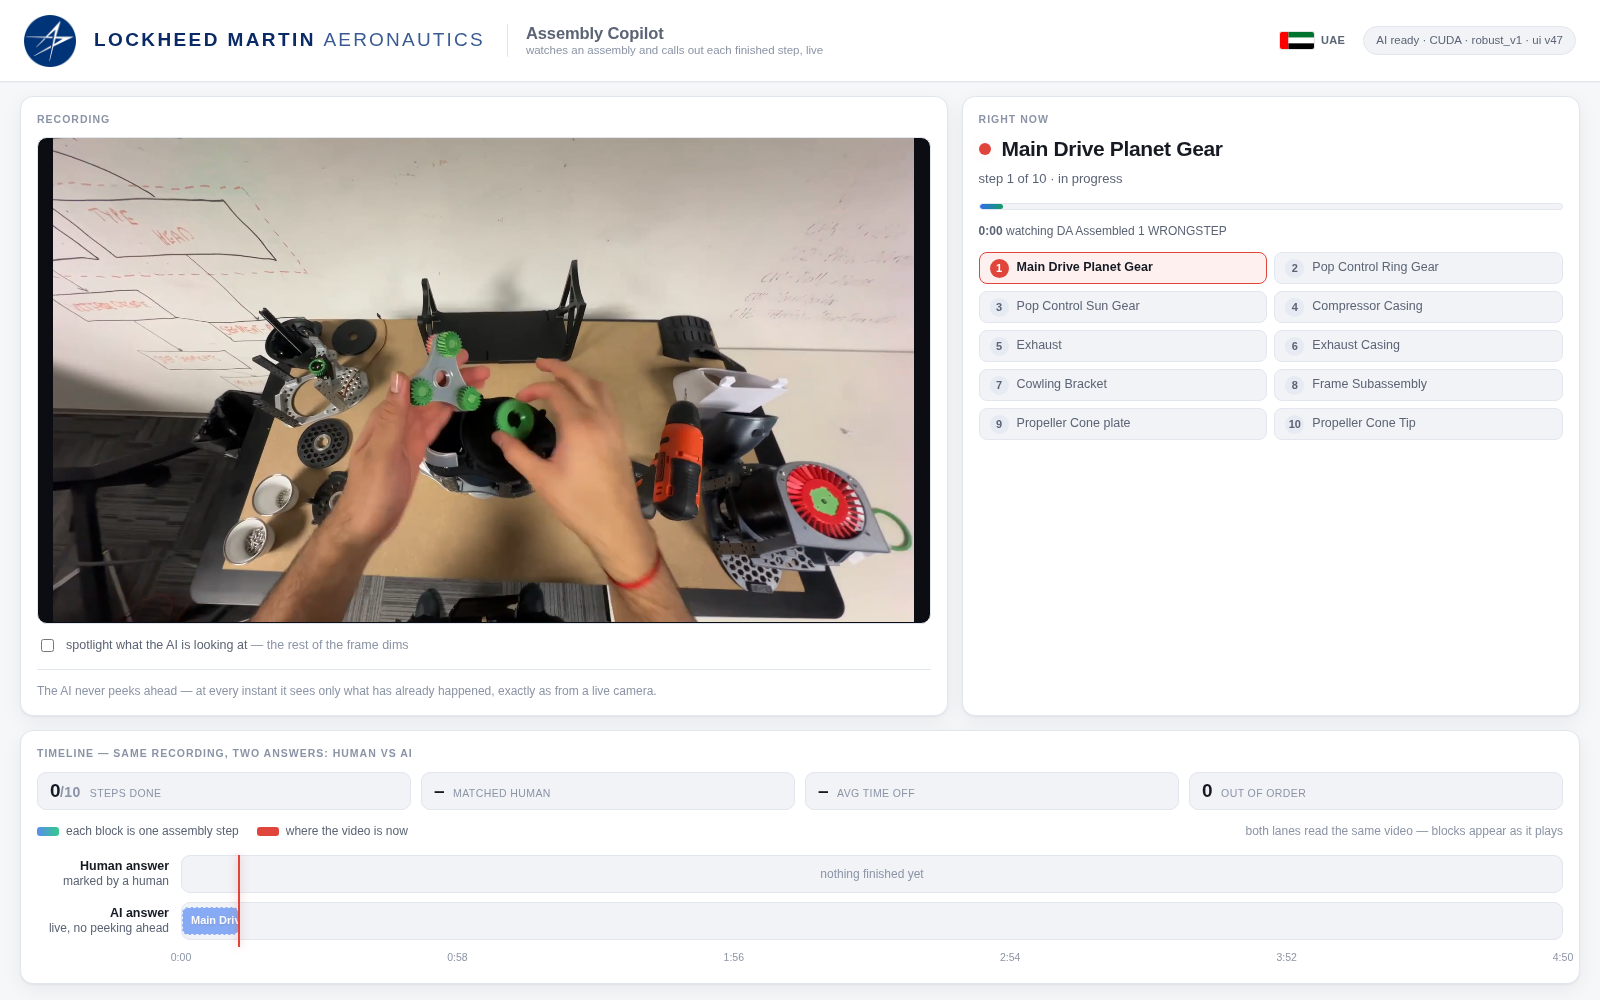
\includegraphics[width=0.98\linewidth]{replay_inference_loaded.png}
\caption{Replay inference interface with an engine-assembly recording loaded. The browser presents the live
recording, current predicted step, ten-step procedure state, progress, and the human-versus-AI timeline. The same
causal head and fixed-lag decoder are used here as in the live serving path.}
\label{fig:replay_ui}
\end{figure}

\begin{table}[H]
\centering
\caption{Served replay verification using the deployed \texttt{robust\_v1} checkpoint. \emph{Steps in place}
counts expected procedure steps recovered by the decoder; these examples are complementary to the aggregate
acceptance-gate scores in Table~\ref{tab:iteration}.}
\label{tab:served_results}
\small
\begin{tabular}{@{}p{0.42\linewidth}rp{0.18\linewidth}@{}}
\toprule
\textbf{Recording} & \textbf{Agreement} & \textbf{Steps in place} \\
\midrule
\texttt{Nahom-Assembled-5} & 93.9\% & 10/10 \\
\texttt{DA-disAssembled-7} & 96.1\% & 10/10 \\
\texttt{Ketan-Assembled-9} & 94.0\% & 10/10 \\
\texttt{Ketan-Assembled-7-SCRAMBLED} & 93.9\% & 10/10 \\
\texttt{DA-Assembled-1-SCRAMBLED} & 91.5\% & 8/8 \\
\texttt{Nahom-Assembled-7-PARTIAL} & 92.5\% & 7/7 \\
\texttt{DA-Assembled-2-REVERSED} & 89.8\% & 10/10 \\
\texttt{Nahom-disAssembled-13-SCRAMBLED} & 85.5\% & 8/9 \\
\bottomrule
\end{tabular}
\end{table}

\subsection{Demo and HoloLens handoff}
\label{sec:demo}

The live demo is intentionally split into a model service and a display client. The
\texttt{holo-lens-api-app} accepts live frames, runs inference, and publishes compact state such as the current
step, expected next step, confidence, progress, warning status, latency, and frame rate. A small overlay publisher
maps the ten model classes to the visible thirteen-part assembly catalogue. Three model classes span two visible
parts, so this mapping is kept in configuration rather than hidden in the network.

The display side is the separate Unity UWP HoloLens application used by the operations-helper project
~\cite{hololensapp}. The local
overlay service receives state changes through \texttt{/step}; the Unity client polls \texttt{/state} and updates
the display. The application contains a scripted demo mode for rehearsals and a live mode for model-driven updates.
The screenshot in Fig.~\ref{fig:hololens_overlay} shows the resulting technician-facing panel with the Lockheed
Martin-branded header, current part, reference image, progress, and telemetry.

The current HoloLens presentation is a movable, resizable 2-D screen-space window rather than a spatially anchored
3-D model overlay. The Unity project uses Microsoft Mixed Reality Toolkit and OpenXR, but the present integration
does not use Vuforia image targets, model targets, or a tracked physical coordinate system. This boundary is useful
for interpreting the demonstration: the model recognizes the procedure and sends state; Unity renders guidance.
Spatial anchoring can be added later without changing the temporal recognition core.

\begin{figure}[H]
\centering
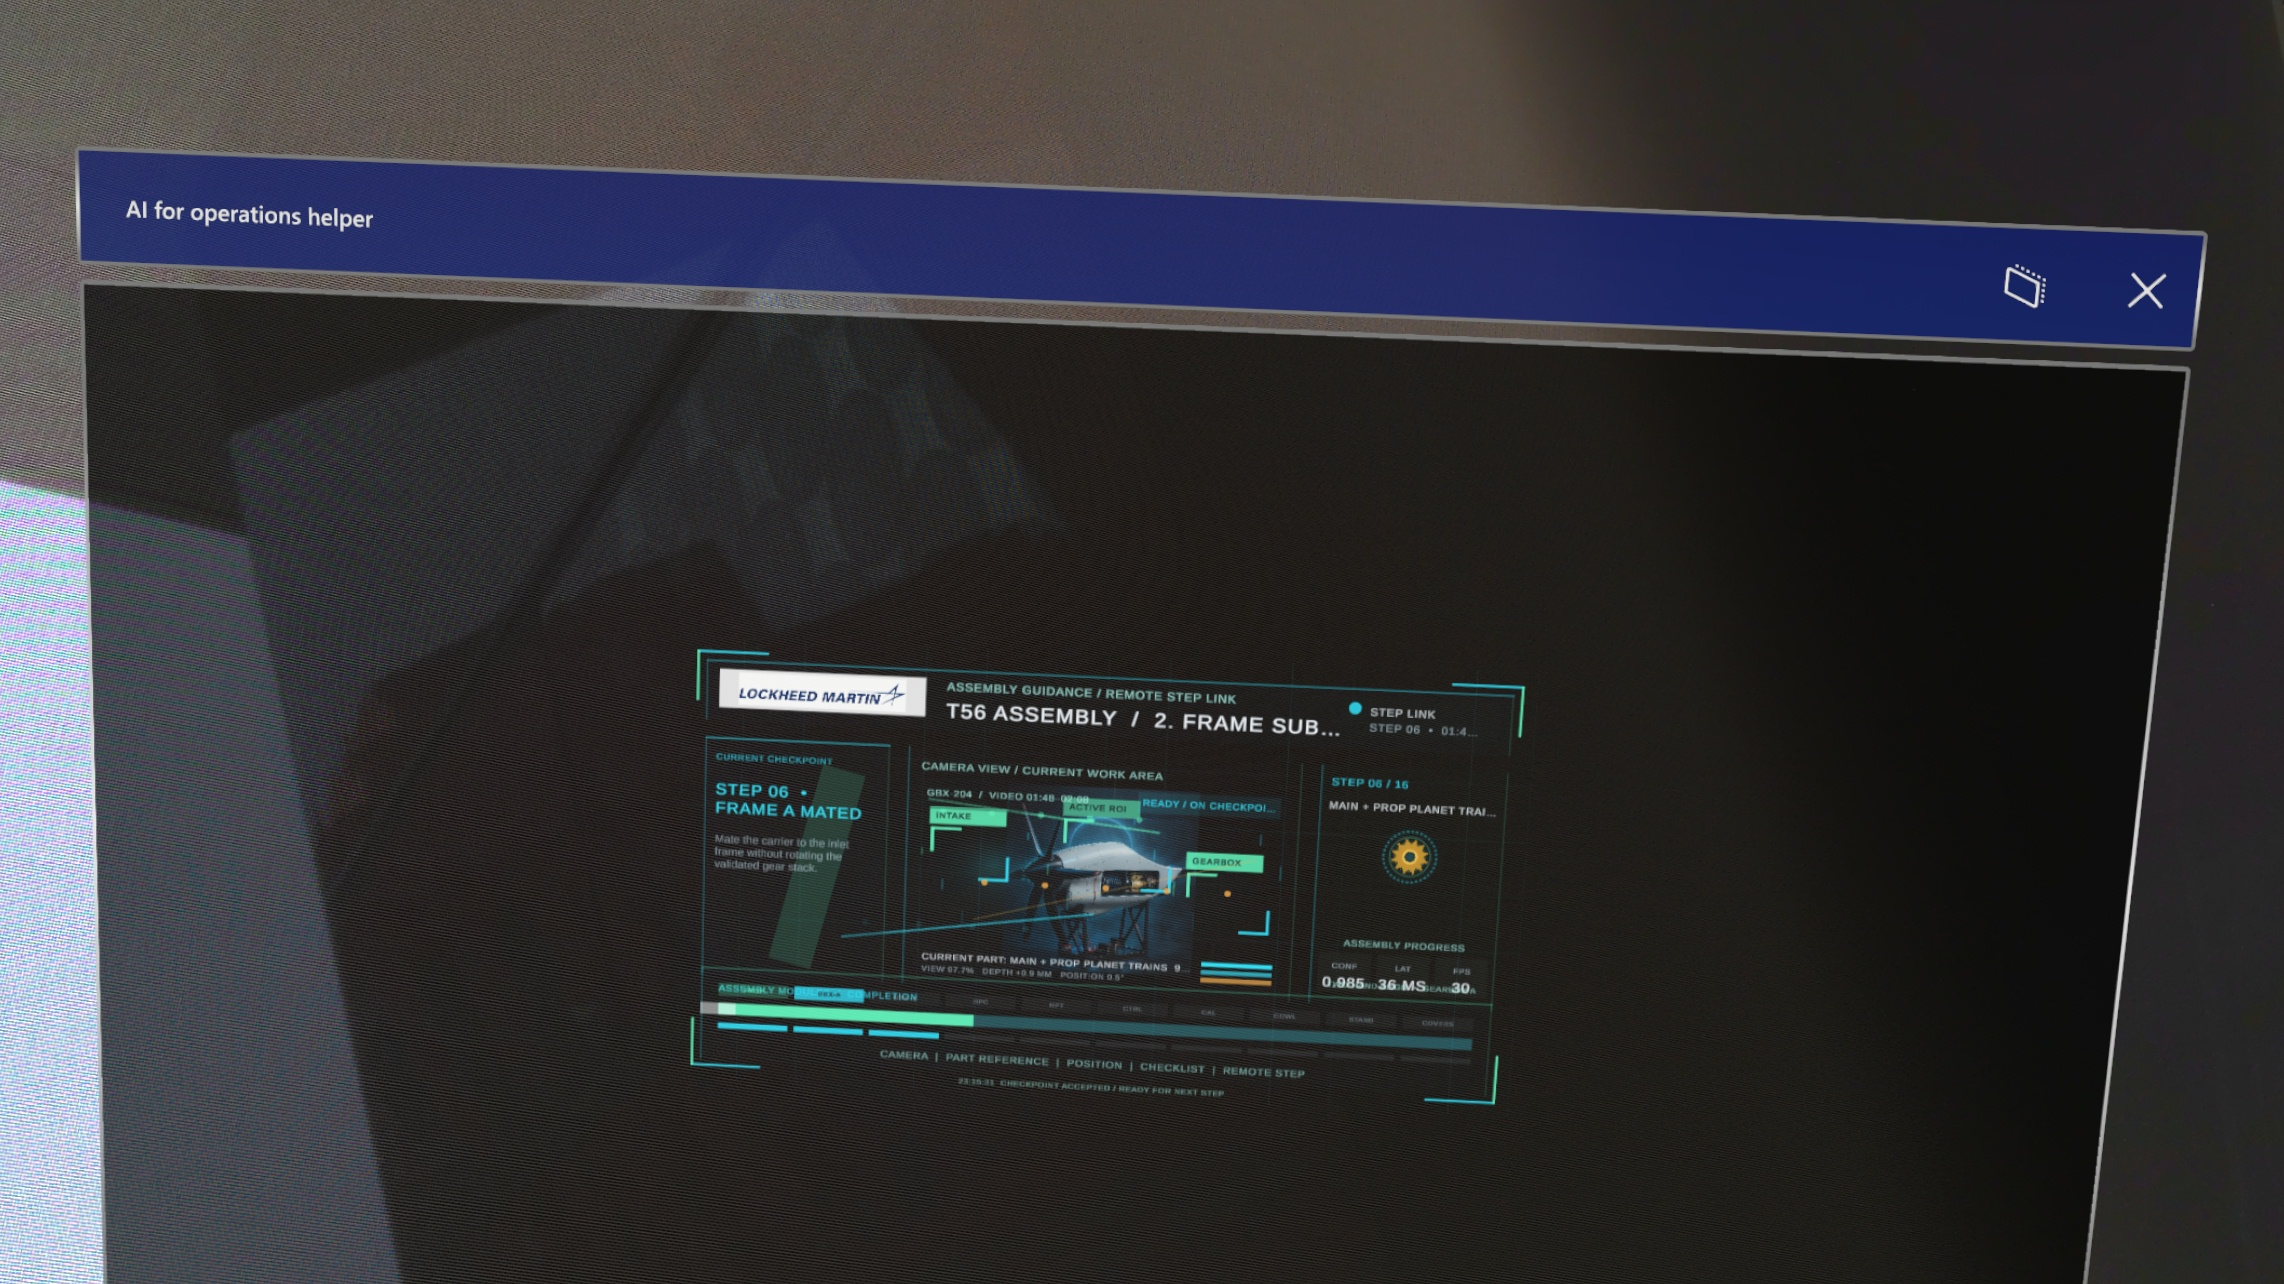
\includegraphics[width=0.84\linewidth]{hololens_overlay.jpg}
\caption{Technician-facing HoloLens overlay used in the live demonstration. The current application renders a
screen-space guidance window and receives compact state updates from the local overlay service; it is not the
recognition model itself and does not currently perform spatial object registration.}
\label{fig:hololens_overlay}
\end{figure}

\subsection{Project structure, reproducibility, and dependencies}
\label{sec:project_structure}

The implementation is organized around the experiment-to-demo flow. The active
\texttt{assembly\_copilot} repository contains the frozen encoders and weights in \texttt{copilot\_model/},
training and acceptance scripts in \texttt{training/}, production annotations and cached features in
\texttt{dataset/}, a browser replay server in \texttt{replay-demo/}, and the live API in
\texttt{holo-lens-api-app/}. The GitLab project suite contains the recording, step-labeling, and optional
component-box labeling applications~\cite{copilottools}. The active repository's
\texttt{REPRODUCING.md} describes the same sequence used during development: prepare features and labels, create
stress videos, train, run the acceptance gate, and finally exercise the served applications
~\cite{copilotrepo}.

The final model assets and dataset metadata are kept with the active project, but the complete demonstration still
has explicit external boundaries. The Python runtime requires the project environment and the video foundation
model dependencies. The live HTTPS path uses certificates and source recordings from the local web-application
workspace. The HoloLens display is a separate Unity 2020.3.28f1 project with MRTK/OpenXR packages and a local
Python overlay service. Recording these boundaries matters for reproducibility: a fresh checkout can reproduce the
model and replay path, while the phone and HoloLens demonstration additionally require the local services and
hardware/display project.

\subsection{Limitations and lessons}
\label{sec:limitations}

Several limitations remain part of the result rather than being hidden by the demo:

\begin{itemize}
  \item The in-house test split is not subject-disjoint, so the reported normal and stress scores are not a
  substitute for evaluation on unseen operators or a new assembly line.
  \item The current causal model recognizes the modeled procedure and its order; it is not yet a general
  wrong-installation judge. A wrong-step stress case tests a useful failure mode, but substantially more
  segment-close incorrect examples are needed for reliable correctness classification.
  \item A committed step is intentionally delayed by the fixed-lag decoder. This trades immediate but unstable
  predictions for announcements that a technician can trust; the measured delay is approximately 2.84\,s.
  \item The model vocabulary and visible overlay vocabulary are not identical: ten learned classes map to thirteen
  displayed parts. This is practical for the current turbofan demonstrator but should be replaced by an explicit
  procedure schema for broader deployments.
  \item The current HoloLens client is a display and interaction surface. It does not yet run the foundation
  encoders on-device or register instructions to physical parts. Future work includes subject-disjoint data,
  richer fault labels, edge optimization, spatial anchoring, and reference-based omission/rework checks.
\end{itemize}

\section{Conclusion}
This work has two connected outcomes. The first is a controlled research study on public procedure-recognition
benchmarks: Viterbi decoding, stronger SSv2-giant features, DiffAct, and two-encoder fusion culminated in
\best{F1@50 $=79.50$}, while the separately reported SAM3-enriched configuration reached $70.1$ and added spatial
enrichment without pretending to solve correctness. The second is
an end-to-end Assembly Copilot built from the lessons of that study. It includes its own egocentric recording and
labeling workflow, a 40-recording turbofan corpus, a causal dual-encoder TCN, fixed-lag online decoding, explicit
order and cold-start stress tests, replay verification, and a live phone-to-HoloLens demonstration path. The
deployed \texttt{robust\_v1} checkpoint achieves 93.06\% on normal held-out data and 90.57\% on scrambled-order
stress data, with a measured 2.84\,s live delay. The clearest next step is to improve data quality and coverage:
subject-disjoint evaluation, more precisely timed incorrect-installation examples, and reference-based checks for
omission, rework, and physical correctness.

\begin{thebibliography}{99}
\small
\bibitem{industreal} T.~Schoonbeek \emph{et al.}, ``IndustReal: A Dataset for Procedure Step Recognition Handling
Execution Errors in Egocentric Videos,'' \emph{WACV}, 2024.
\bibitem{meccano} F.~Ragusa \emph{et al.}, ``The MECCANO Dataset: Understanding Human-Object Interactions from
Egocentric Videos in an Industrial-like Domain,'' \emph{WACV}, 2021.
\bibitem{mstcn} Y.~A.~Farha and J.~Gall, ``MS-TCN: Multi-Stage Temporal Convolutional Network for Action
Segmentation,'' \emph{CVPR}, 2019.
\bibitem{asformer} F.~Yi, H.~Wen, and T.~Jiang, ``ASFormer: Transformer for Action Segmentation,'' \emph{BMVC}, 2021.
\bibitem{diffact} D.~Liu \emph{et al.}, ``Diffusion Action Segmentation,'' \emph{ICCV}, 2023.
\bibitem{videomae} L.~Wang \emph{et al.}, ``VideoMAE V2: Scaling Video Masked Autoencoders with Dual Masking,''
\emph{CVPR}, 2023.
\bibitem{internvideo2} Y.~Wang \emph{et al.}, ``InternVideo2: Scaling Video Foundation Models for Multimodal Video
Understanding,'' \emph{ECCV}, 2024.
\bibitem{miniroad} S.~An \emph{et al.}, ``MiniROAD: Minimal RNN Framework for Online Action Detection,''
\emph{ICCV}, 2023.
\bibitem{testra} Y.~Zhao and P.~Kr\"ahenb\"uhl, ``Real-Time Online Video Detection with Temporal Smoothing
Transformers,'' \emph{ECCV}, 2022.
\bibitem{sam} A.~Kirillov \emph{et al.}, ``Segment Anything,'' \emph{ICCV}, 2023.
\bibitem{sam2} N.~Ravi \emph{et al.}, ``SAM 2: Segment Anything in Images and Videos,'' \emph{arXiv:2408.00714}, 2024.
\bibitem{sam3} Meta AI, ``SAM 3: Segment Anything with Concepts,'' Technical Report / \texttt{facebook/sam3}, 2025.
\bibitem{locateanything} NVIDIA, ``LocateAnything-3B: A Grounding Vision-Language Model,''
\texttt{nvidia/LocateAnything-3B}, 2025.
\bibitem{qwen25} Qwen Team, ``Qwen2.5 Technical Report,'' \emph{arXiv:2412.15115}, 2024.
\bibitem{copilotrepo} Assembly Copilot project, \emph{README and REPRODUCING.md}, internal project repository,
2026.
\bibitem{copilottools} Assembly Copilot project suite, \emph{assembly\_video\_recorder,
assembly\_video\_labeler, and box\_part\_labeler}, internal GitLab repository, 2026.
\bibitem{hololensapp} AI for Operations Helper, \emph{HoloLens Operations Helper Overview and Model Integration
Handoff}, internal Unity project documentation, 2026.
\end{thebibliography}

\end{document}
